\documentclass[11pt]{article}

\usepackage{extras} % Se extras.sty
\usepackage{tikz}
\usepackage{graphicx}
\usepackage{epstopdf}


\begin{document}
\begin{titlepage}
\begin{center}

{\Large\bfseries TSEA56 - Kandidatprojekt i elektronik \\ LIPS Förstudie: Sensor}

\vspace{5em}

Version 0.1

\vspace{5em}
Grupp 4 \\
\begin{tabular}{rl}
Wasteson, Emil&\verb+emiwa068+
\\
Inge, Zimon&\verb+zimin415+
\\
\end{tabular}

\vspace{5em}
\today

\vspace{16em}
Status
\begin{longtable}{|l|l|l|} \hline

Granskad & - & - \\ \hline
Godkänd & - & - \\ \hline
 
\end{longtable}

\end{center}
\end{titlepage}

\pagebreak
\begin{center}

\section*{PROJEKTIDENTITET}
2016/VT, Undsättningsrobot Gr. 4

Linköpings tekniska högskola, ISY
\vspace{5em}
\begin{center}

\begin{tabular}{|l|l|l|l|} \hline
\textbf{Namn} & \textbf{Ansvar} & \textbf{Telefon} & \textbf{E-post}  \\ \hline 
Isak Strömberg (IS) & Projektledare & 073-980 38 50 & isast763@student.liu.se \\ \hline
Olle Hynén Ulfsjöö (OHU)& Dokumentansvarig & 070-072 91 84 & ollul666@student.liu.se \\ \hline
Emil Wasteson (EW) & Hårdvaruansvarig & 076-836 61 66 & emiwa068@student.liu.se \\ \hline
Elena Tronje (ET) & Mjukvaruansvarig & 072-276 92 93 & eletr654@student.liu.se \\ \hline
Zimon Inge (ZI)& Testansvarig & 070-171 35 18 & zimin415@student.liu.se \\ \hline
Lovisa Gustafsson (LG) & Leveransansvarig & 070-210 32 53 & lovgu777@student.liu.se \\ \hline
\end{tabular}

\end{center}

E-postlista för hela gruppen: isast763@student.liu.se

\vspace{5em}
Kund: ISY, Linköpings universitet \\
tel: 013-28 10 00, fax: 013-13 92 82 \\
Kontaktperson hos kund: Mattias Krysander \\
tel: 013-28 21 98, e-post: matkr@isy.liu.se \\

\vspace{5em}
Kursansvarig:  Tomas Svensson\\
tel: 013-28 13 68, e-post: tomass@isy.liu.se \\
Handledare: Peter Johansson \\
tel: 013-28 13 45, e-post: peter.a.johansson@liu.se
\end{center}
\pagebreak

\tableofcontents

\pagebreak
\section*{Dokumenthistorik}
\begin{table}[h]
\begin{tabular}{|l|l|l|l|l|} \hline

\textbf{Version} & \textbf{Datum} & \textbf{Utförda förändringar} & \textbf{Utförda av} & \textbf{Granskad} \\ \hline
0.1 & - &  Första utkastet & Grupp 4 & - \\ \hline
\end{tabular}
\end{table}

\pagebreak
\pagenumbering{arabic}

\begin{flushleft}

\section{Inledning}
I dagsläget finns det en mängd olika sensorer, alla med för- respektive nackdelar. Vilken sensor som är bäst beror ofta på vilket syfte som ska uppfyllas och vilka resurser som finns att tillgå. Att en undsättningsrobot som ska hitta nödställda har sensorer som gör det enkelt att identifiera sitt mål är en fråga om liv och död. Därav finns det ett stort behov av att öka kunskapen om sensorer, samt dess möjligheter och begränsningar.

\pagebreak

\section{Problemformulering}

\subsection{Syfte}
Syftet med denna rapport är att undersöka vilka sensorer som är relevanta för undsättningsroboten i sitt uppdrag. Syftet är fortsättningsvis att redogöra för en implementation av de sensorer som finnes intressanta för undsättningsrobotens ändamål.


\subsection{Frågeställningar}
Nedan följer de huvudsakliga frågeställningar vilka har för avsikt att behandlas i denna rapport:



\begin{itemize}
	\item	 Vilka sensorer finns det som stöd för att roboten ska kunna utföra sitt uppdrag? Hur fungerar dessa? Finns det olika typer?
	\item Vilka sensorer är lämpliga att använda till projektet?
	\item 

Hur kan dessa implementeras? 
\end{itemize}



\pagebreak

\section{Kunskapsbas}
I följande avsnitt följer en beskrivning av olika typer av sensorer.

\subsection{Kapacitiv sensor}
En kapacitiva sensor är en sensor som använder sig av kapacitans (C) för att identifiera ett önskat material. Sensorn består av en platta med arean A och kan detektera alla objekt som har en relativ kapacivitet som skiljer sig från luft, bland annat plast, olika metaller, vätskor och hud. Det finns olika typer av kapacativa sensorer, en del kräver kontakt mellan sensorn och ett objekt medan andra har högre känslighet och kan känna av kapacitansändringar på avstånd upp till 70 cm. (2)

%http://www.capsense.com/capsense-wp.pdf (2)

\subsubsection{FDC1004}
En sensor som inte kräver kontakt är FDC1004. Det kan implementeras med hjälp av en I\textsuperscript{2}C-buss och kan känna igen olika typer av material. När avståndet (d) mellan objektet och en sensorn minskar så ökar kapacitansen enligt ekvation 1, där er är en konstant som beror av materialets relativa kapacivitet och eo är en permitiviteten i luften. (1), (3)

\begin{equation*}
	\textrm{C} = \frac {e_{r} \times e_{o} \times A}{d}						
\end{equation*}

I figur 4 illustreras hur kapacitansen ändras när objektet (fingret) närmar sig sensorn och hur kapacitansändringen med hjälp av en AD-omvandlare görs om till en digital signal. 

\begin{figure}[htbp]
	\centering
	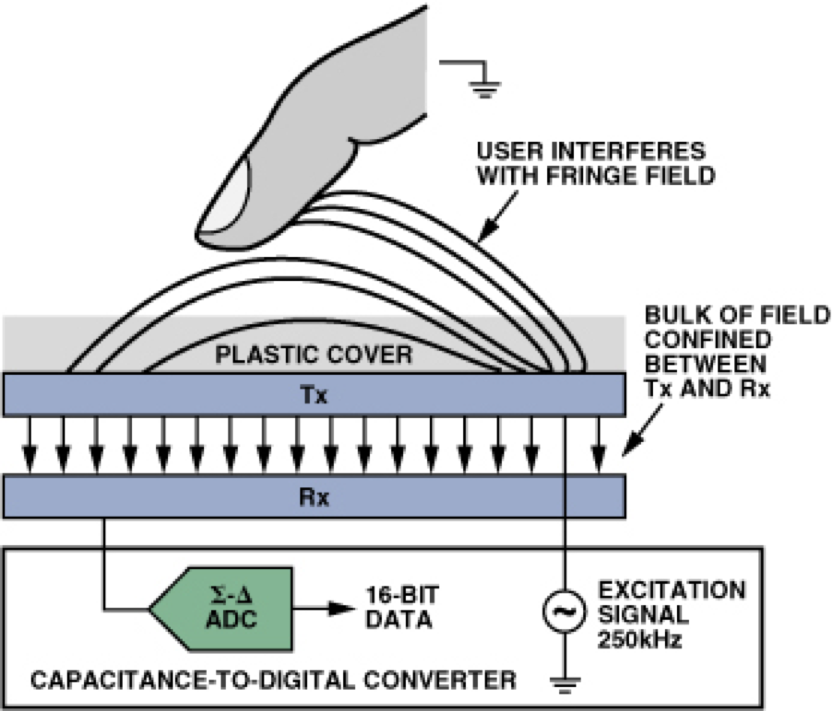
\includegraphics[scale=0.4]{Images/capacative}
	\caption{Ett fingers påverkan på kapacitans \label{capacative}}
\end{figure}

Förhållandet mellan kapacitans och spänning visas i figur 2.

\begin{figure}[htbp]
	\centering
	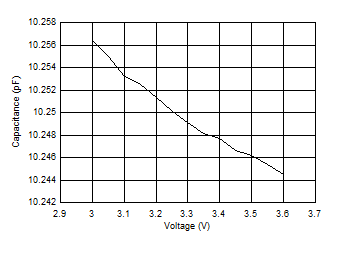
\includegraphics[scale=0.8]{Images/capacitance_voltage}
	\caption{Förhållande mellan analog spänning och kapacitans \label{capacitance_voltage}}
\end{figure}


% http://www.ti.com/lit/ds/symlink/fdc1004.pdf (1)

%http://www.ti.com/lit/an/snoa927/snoa927.pdf (3)


\subsection{Ultraljudssensorer}
För att mäta avstånd till objekt kan en ultraljudssensor användas. Den skickar ut en puls av ljud, utanför det intervall människan kan uppfatta, för att sedan invänta ett eventuellt eko. Om inget eko detekteras finns det inget objekt inom sensorns avkänningsområde i den riktning som ljudpulsen skickades ut i. Uppfattas däremot ett eko registrerar sensorn hur lång tid (t) det tog för ljudet att studsa tillbaka och kan, eftersom ljudhastigheten (vluft) i luft är känd, utifrån det enligt ekvation 2 räkna ut avståndet (s) till det objekt som gav upphov till ekot. 

\begin{equation*}
	\textrm{s} = v_{luft} \times t						
\end{equation*}

\subsubsection{SRF04}
Ultraljudssensorn SRF04 mäter avstånd mellan 3 cm och 3 meter med hjälp av ultraljud. Den har en detektionskon på ca 30 grader, vilket gör att den kan upptäcka objekt trots att ekot inte studsar optimalt (vinkelrätt) mot ett objekt och den implementeras enkelt med en I\textsuperscript{2}C-buss. (1)

%https://docs.isy.liu.se/pub/VanHeden/DataSheets/srf04.pdf (1)


\subsection{Ljussensor}
En ljussensor består av en högresistiv halvledare vilken absorberar fotoner. Baserat på mängden fotoner sensorn absorberar och frekvensen på dessa så ges det halvledande materialets bundna elektroner tillräckligt med energi för att göra en förflyttning till ledningsbandet. De fria elektronerna medför sedermera att elektrisitet leds,  vilket i sin tur resulterar i att variaritioner i ljussensorns motstånd. Detta innebär att motståndet hos en ljussensor är högt i mörker, för att sedan minska i ljusare miljöer. \cite{612896}

Ljussensorn (även kallad fotocell) omvandlar följaktligen infallande ljus till elektrisk ström där strömstyrkan varierar beroende ljusets styrka. Av denna anledning så är en ljussensor användbar vid detektering av konstraster på exempelvis en yta.

En reflektorfotocell är en typ av ljussensor som, liksom ljussensorn, detekterar förändringar i ljusintensiteten. Det typiska i reflektorfotocellen är dock att den  består av en ljuskälla, en motagare, en signalkonverterare och slutligen en förstärkare. \cite{reflective}

%http://www.automation.com/library/articles-white-papers/sensors-sensing-technologies/fundamentals-of-photoelectric-sensors (1)




\subsubsection{Zimon}


\subsection{IR-sensor}
En IR-sensor är en tillämpning av en ljussensor som endast registrerar önskade våglängder i det infraröda spektrumet. I figur 1 illustreras hur en sensor, med hjälp av en LED-lampa som sänder ut strålning med samma våglängd som den sensorn uppfattar, kan avgöra om ett det finns ett objekt i sensorns riktning. Detekteras reflekterad strålning betyder det att ett föremål finns i sensorns riktning. (1)

\begin{figure}[htbp]
	\centering
	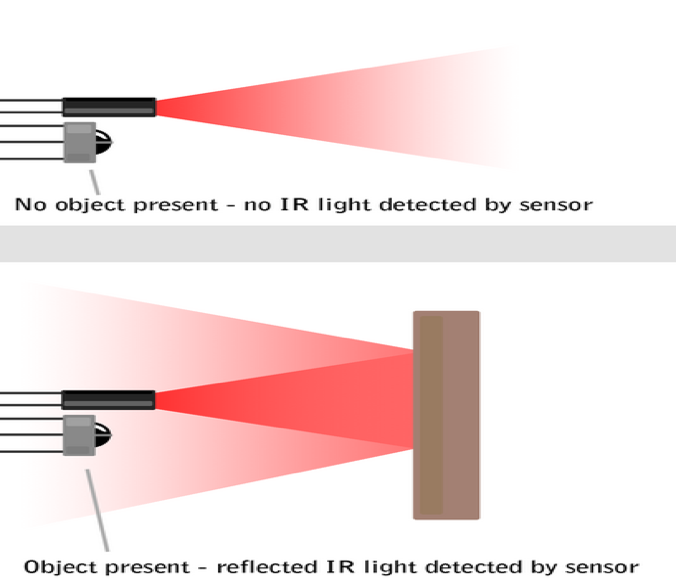
\includegraphics[scale=0.4]{Images/Laser}
	\caption{Illustration av lasersensor \label{Laser}}
\end{figure}

Det går även att använda som en avståndssensor, vilket illustreras i figur 2, genom att sensorn mäter vinkeln av det reflekterade ljuset som strålningen av LED-lampan ger upphov till. Detta ställer högre krav på sensorn, eftersom strålningen behöver vara skarpare.

\begin{figure}[htbp]
	\centering
	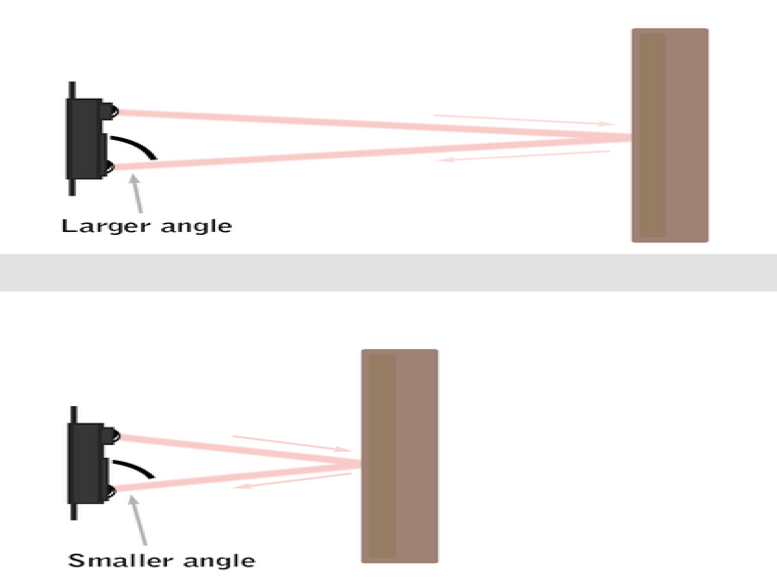
\includegraphics[scale=0.4]{Images/laser_angle}
	\caption{Vinkelmätning med lasersensor \label{laser_angle}}
\end{figure}

Ytterligare en möjlighet med en IR-sensor är att mäta hur ljusskillnader. Eftersom ljusa objekt reflekterar mer ljus än vad mörka gör kan sensorn reagera på reflektioner mot ett ljust objekt, men inte mot ett mörkt.

%http://education.rec.ri.cmu.edu/content/electronics/boe/ir_sensor/1.html (1)

\subsubsection{IRM-8601-S}


\subsubsection{GP2D120}

\subsection{Lasersensor}
Det finns olika typer av lasersensorer som använder olika tekniker foch har olika funktioner. En typ är den avståndsmätande elektrooptiska sensorn som sänder ut en laser stråle och mäter hur lång tid (t) det tar innan den reflekteras och detekteras av sensorn. Avståndet (D) är räknas fram enligt ekvation 1, där c står för ljusets hastighet i luft.

\begin{equation*}
	\textrm{D} = \frac {c \times t}{2}						
\end{equation*}

En annan typ av lasersensor är den triangulerade sensorn. De är mer komplex och kan mäta avstånd på ett mer precist sätt än den elektrooptiska. 

%http://www.mtiinstruments.com/pdf/appnotes/lasersensor.pdf (1)

\subsubsection{LIDAR-Lite}


\subsection{Gyro-/accelerometer}

\pagebreak
\section{Rapportens huvuddel, byt rubriknamn}
text

\section{Resultat och slutsatser}
text

\pagebreak
\addcontentsline{toc}{section}{Referenser}




\pagebreak
\appendix
\section{First Appendix}

\end{flushleft}

\bibliographystyle{ieeetr}
\bibliography{references}
\end{document}